\chapter{KI}
Nedenfor følger design af software til Kontrolinterfacet. Dette er lavet på baggrund af kravspecifikation og systemarkitektur. 
\subsection{Modulets ansvar}
Kontrolinterfacet er brugerens primære kontaktflade til systemet. Programmet indeholder en brugergrænseflade der opfylder kravene i Kravspecifikationen. Her kan der også ses en prototype på den grafiske brugergrænseflade.
Kontrolinterfacet står for at modtage inputs fra brugeren. Disse inputs sendes som kommandoer til Styringsmodulet. Det er også herfra at Kontrolinterfacet modtager de værdier, som sidenhen vises på den grafiske brugergrænseflade. Kontrolinterfacet står også for kommunikationen til den eksterne database. Her sendes en række parametre om skibet og dets status.
\subsection{Klassediagram}
Nedenfor ses klassediagrammet for Kontrolinterfacet. Bemærk at klassediagrammet er delt op i to. Skæringsstedet er mellem Kontrolinterface-klassen og Styringsmodul-klassen og er markeret med <<extend>>.

\begin{figure}[H]
\centering
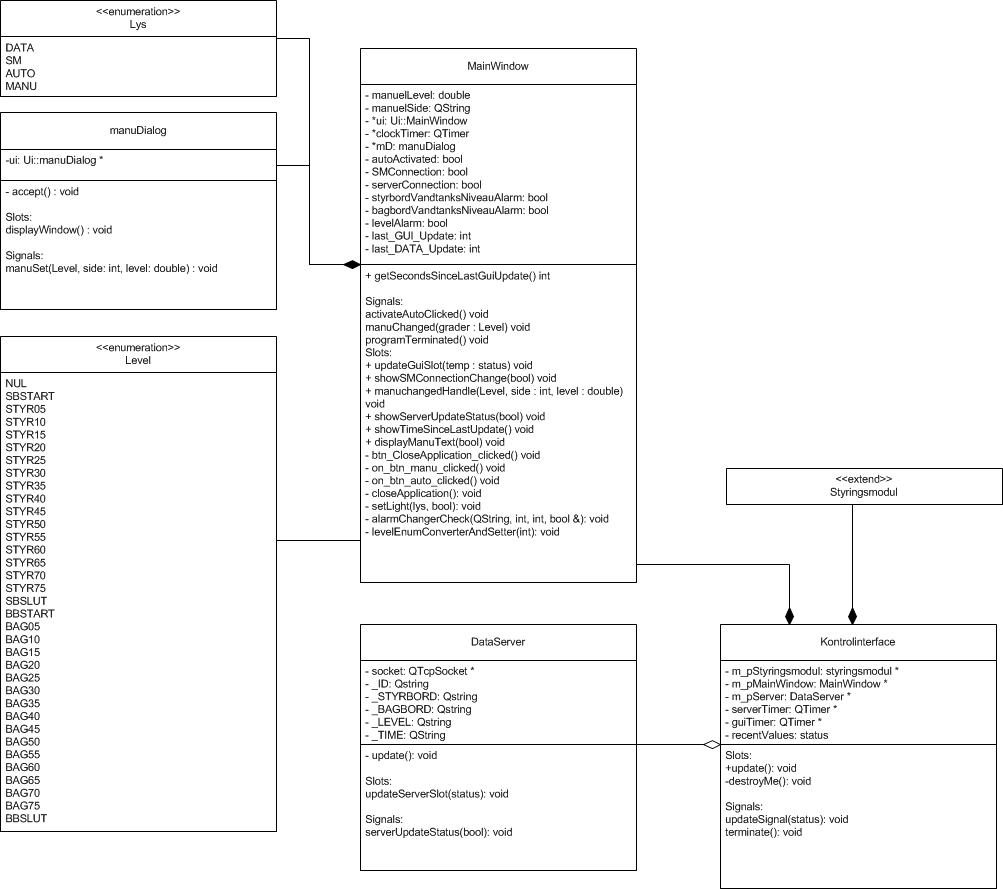
\includegraphics[width=1\textwidth]{billeder/KI-Class}
\caption{På figuren ses klassediagrammet for KI - Kontrolinterface-delen}
\end{figure}

\begin{figure}[H]
\centering
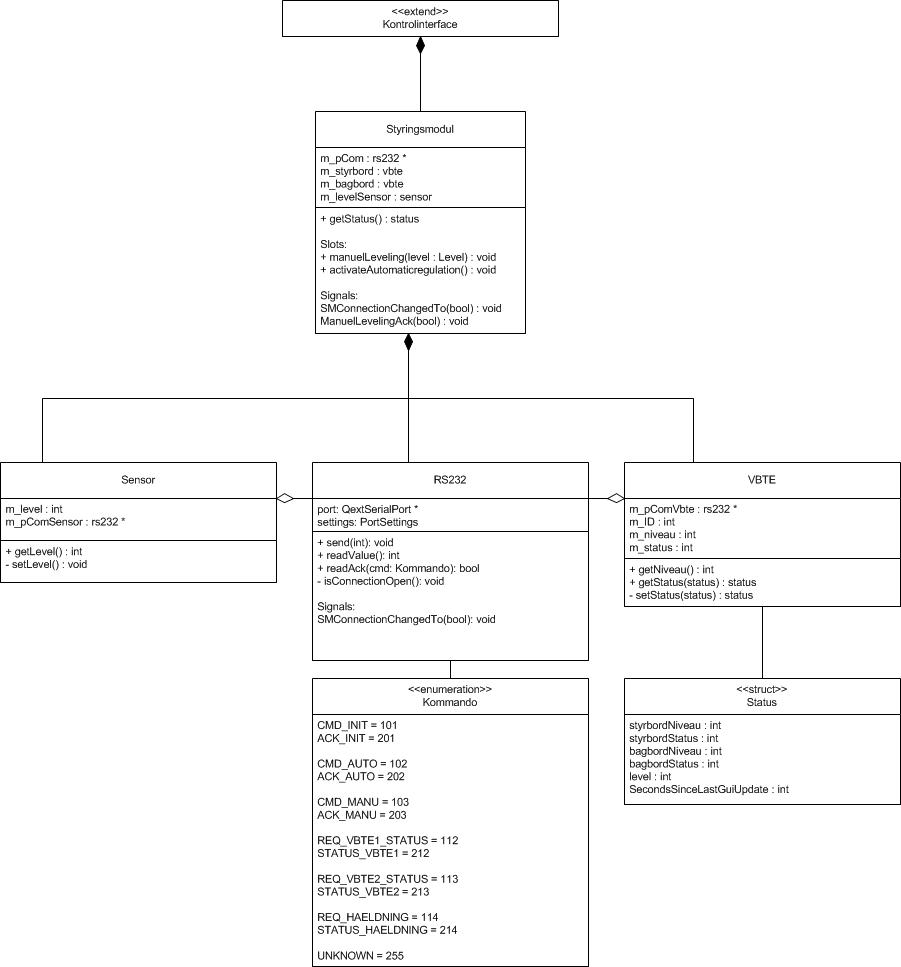
\includegraphics[width=1\textwidth]{billeder/SM-Class}
\caption{På figuren ses klassediagrammet for KI - Styringsmodul-delen}
\end{figure}

\section{Metode- og klassebeskrivelser}
\subsection{MainWindow}
\subsubsection{Ansvar}
Denne klasse indeholder de funktioner der er skrevet til Qt-formen MainWindow.ui hvori selve det grafiske er opbygget. Klassen indeholder de funktioner der anvendes i forbindelse med den grafiske brugergrænseflade. Det være sig når der kommer et input, eller der skal opdateres nogle værdier på skærmen.
\subsubsection{Funktionsbeskrivelser}
 
\begin{table}[H]
\begin{tabular}{l p{12.5cm}}
\multicolumn{2}{l}{\texttt{\textcolor{blue}{int} getSecondsSinceLastGuiUpdate();}} \\
\hline
Beskrivelse:& En simpelt get-funktionen der returnerer værdien af klasseattributten \textit{last\_GUI\_Update.} \\
Parametre:&Ingen\\
Returværdi:&\texttt{\textcolor{blue}{int} secondsSinceLastGuiUpdate}\\
\end{tabular}
\end{table}

\begin{table}[H]
\begin{tabular}{l p{12.5cm}}
\multicolumn{2}{l}{\texttt{\textcolor{blue}{void} updateGuiSlot(status temp);}} \\
\hline
Beskrivelse:& Bliver kaldt når GUI'en skal opdateres. 
Den modtager parameterent \textit{temp} som er en struct af typen status. 
Ud fra denne struct hives de værdier ud, som skal vises på GUI'en. Værdierne vises ved de set-funktioner der er tilknyttet de anvendte widgets (og dermed en del af Qt-frameworket.) 
Når værdierne er opdateret vises det som en aktivitet i aktivitetsloggen \\   
Parametre:&\texttt{\textcolor{blue}{status} temp}\\
Returværdi:&Ingen\\
\end{tabular}
\end{table}

\begin{table}[H]
\begin{tabular}{l p{12.5cm}}
\multicolumn{2}{l}{\texttt{\textcolor{blue}{void} showSMConnectionChange();}} \\
\hline
Beskrivelse:& Kaldes hvis SM-forbindelsen til styringsmodulet ændres fra forbundet til mistet forbindelse eller omvendt. Det udløser en aktivitet i aktivitetsloggen. Derudover skiftes lyset på gui'en. Parameteren state er den status som forbindelsen har ændret sig til.\\   
Parametre:&\texttt{\textcolor{blue}{bool} state}\\
Returværdi:&Ingen\\
\end{tabular}
\end{table}

\begin{table}[H]
\begin{tabular}{l p{12.5cm}}
\multicolumn{2}{l}{\texttt{\textcolor{blue}{void} manuChangedHandle(Level samlet, int side, double level);}} \\
\hline
Beskrivelse:& Kaldes når brugeren har ændret i indstillingen til den manuelle hældning. Som parametre modtages hvilken side man ønsker at skibet skal hælde til (int side), hvor meget det skal hælde (double level) samt de to informationer samlet i en enum, Level samlet.
Funktionen emitter signalet "manuChanged(Level temp). Det sætter også klasseattributerne manuelSide, manuelLevel samt autoActivated til deres rette værdier.
Til sidst kaldes funktionen displayManuText(true)\\   
Parametre:&\texttt{\textcolor{blue}{Level} samlet}\\
&\texttt{\textcolor{blue}{int} side}\\
&\texttt{\textcolor{blue}{double} level}\\
Returværdi:&Ingen\\
\end{tabular}
\end{table}


\begin{table}[H]
\begin{tabular}{l p{12.5cm}}
\multicolumn{2}{l}{\texttt{\textcolor{blue}{void} showServerUpdateStatus(bool state);}} \\
\hline
Beskrivelse:&Kaldes hver gang signalet DataServer::serverUpdateStatus() udsendes. Funktionen undersøger om forbindelsen har ændret sig ved at sammenligne med attributen serverConnection.
Hvis forbindelsen har ændret sig udsendes dette som en aktivitet. Lyset ændres også således at det passer ved hjælp af setLight(DATA, serverConnection. Hvis vi modtager "true" vil last\_DATA\_Update opdateres til således til den nuværende værdi af sekunder siden epoch.\\   
Parametre:&Ingen\\
Returværdi:&Ingen\\
\end{tabular}
\end{table}


\begin{table}[H]
\begin{tabular}{l p{12.5cm}}
\multicolumn{2}{l}{\texttt{\textcolor{blue}{void} showTimeSinceLastUpdate();}} \\
\hline
Beskrivelse:&Kaldes hvert sekund. Funktionen opdaterer antallet af sekunder siden sidste overførelse af data til serveren eller til SM. Når tiden er længere end tiden mellem hver opdatering vil dette tal skifte til rødt.\\    
Parametre:&Ingen\\
Returværdi:&Ingen\\
\end{tabular}
\end{table}


\begin{table}[H]
\begin{tabular}{l p{12.5cm}}
\multicolumn{2}{l}{\texttt{\textcolor{blue}{void} displayManuText(bool show);}} \\
\hline
Beskrivelse:&Viser eller skjuler teksten med indstillingen af manuel hældning afhængig af parameteret show.\\    
Parametre:&Ingen\\
Returværdi:&Ingen\\
\end{tabular}
\end{table}



\begin{table}[H]
\begin{tabular}{l p{12.5cm}}
\multicolumn{2}{l}{\texttt{\textcolor{blue}{void} activateAutoClicked();}} \\
\hline
Beskrivelse:& udsendes når der er blevet trykket på knappen \textit{activateAutoClicked}\\
Parametre:&Ingen\\
Returværdi:&Ingen\\
\end{tabular}
\end{table}


\begin{table}[H]
\begin{tabular}{l p{12.5cm}}
\multicolumn{2}{l}{\texttt{\textcolor{blue}{void} activateAutoClicked();}} \\
\hline
Beskrivelse:& udsendes når der er blevet trykket på knappen \textit{activateAutoClicked}\\
Parametre:&Ingen\\
Returværdi:&Ingen\\
\end{tabular}
\end{table}


\begin{table}[H]
\begin{tabular}{l p{12.5cm}}
\multicolumn{2}{l}{\texttt{\textcolor{blue}{void} manuChanged(Level grader);}} \\
\hline
Beskrivelse:&Udsendes når der er blevet ændret en manuel indstilling.\\
Parametre:&\texttt{\textcolor{blue}{Level} grader}\\
Returværdi:&Ingen\\
\end{tabular}
\end{table}


\begin{table}[H]
\begin{tabular}{l p{12.5cm}}
\multicolumn{2}{l}{\texttt{\textcolor{blue}{void} programTerminated();}} \\
\hline
Beskrivelse:&Udsendes når programmet er blevet lukket ned.\\
Parametre:&Ingen\\
Returværdi:&Ingen\\
\end{tabular}
\end{table}

\begin{table}[H]
\begin{tabular}{l p{12.5cm}}
\multicolumn{2}{l}{\texttt{\textcolor{blue}{void} btn\_CloseApplication\_clicked();}} \\
\hline
Beskrivelse: &Kaldes når luk-knappen på GUI'en er blevet trykket. 
Udsender signalet programTerminated() hvis brugeren bekræfter valget\\
Parametre:&Ingen\\
Returværdi:&Ingen\\
\end{tabular}
\end{table}

\begin{table}[H]
\begin{tabular}{l p{12.5cm}}
\multicolumn{2}{l}{\texttt{\textcolor{blue}{void} on\_btn\_manu\_clicked();}} \\
\hline
Beskrivelse: &Kaldes når der bliver trykket på knappen for manuel hældning. Viser dialogen "manuDialog".\\
Parametre:&Ingen\\
Returværdi:&Ingen\\
\end{tabular}
\end{table}

\begin{table}[H]
\begin{tabular}{l p{12.5cm}}
\multicolumn{2}{l}{\texttt{\textcolor{blue}{void} on\_btn\_auto\_clicked();
}} \\
\hline
Beskrivelse:&Kaldes når der trykkes på \textit{Automatisk Hældnings-knappen}. Aktiverer automatisk styring og deaktiverer den manuelle.\\
Parametre:&Ingen\\
Returværdi:&Ingen\\
\end{tabular}
\end{table}

\begin{table}[H]
\begin{tabular}{l p{12.5cm}}
\multicolumn{2}{l}{\texttt{\textcolor{blue}{void} setLight(lys id, bool state);}} \\
\hline
Beskrivelse:&Sætter lyset i forhold til parametrene. lys er en enum der bestemmer hvilket element lyset skal ændres for. state er om lyset skal være tændt eller ej\\
Parametre:&\texttt{\textcolor{blue}{lys} id}\\
&\texttt{\textcolor{blue}{bool} state}\\
Returværdi:&Ingen\\
\end{tabular}
\end{table}

%\multicolumn{2}{l}{\texttt{\textcolor{blue}{void} alarmChangerCheck(QString sentence, int critical\_point, int value, bool &earlier\_state);}} \\

\begin{table}[H]
\begin{tabular}{l p{12.5cm}}
\multicolumn{2}{l}{\texttt{\textcolor{blue}{void} alarmChangerCheck(QString sentence, int critical\_point, int value, bool \&earlier\_state);}} \\
\hline
Beskrivelse: &Tester om alarmerne har ændret sig. Sentence er starten af den sætning der skrives i aktivitetsloggen. critical\_point er det kritiske punkt for det emne der arbejdes på. Value er den værdi den har. Earlier\_state er hvilket stadie alarmen var i tidligere.\\
Parametre:&\texttt{\textcolor{blue}{QString} sentence}\\
&\texttt{\textcolor{blue}{int} critical\_point}\\
&\texttt{\textcolor{blue}{int} value}\\
&\texttt{\textcolor{blue}{bool} \&earlier\_state}\\
Returværdi:&Ingen\\
\end{tabular}
\end{table}

\begin{table}[H]
\begin{tabular}{l p{12.5cm}}
\multicolumn{2}{l}{\texttt{\textcolor{blue}{void} levelEnumConverterAndSetter(int level);}} \\
\hline
Beskrivelse: &Konverterer en integer baseret på Level-enumeratoren om til en side og en vinkel.\\
Parametre:&\texttt{\textcolor{blue}{int} level}\\
Returværdi:&Ingen\\
\end{tabular}
\end{table}


\subsection{Kontrolinterface}
\subsubsection{Ansvar}
Dette er hovedklassen hvori selve programmet lever. Oprettelsen af et objekt af denne klasse er derfor også det eneste der sker i main.
\subsubsection{Funktionsbeskrivelser}

\subsection{DataServer}
\subsubsection{Ansvar}
Klassen står for al kommunikation med serveren via en TCP-forbindelse. Forbindelse oprettes og nedlægges hver gang der tages kontakt. DataServer-objektet opdaterer serveren når den får ordre om det fra Kontrolinterface-klassen.
\subsubsection{Funktionsbeskrivelser}

\subsection{manuDialog}
\subsubsection{Ansvar}
manuDialog-klassen står for håndtering af det vindue der åbnes ved tryk på \textit{Manuel Hældningsregulering-knappen}.
\subsubsection{Funktionsbeskrivelser}

\subsection{Styringsmodul}
\subsubsection{Ansvar}
Klassen har samme rolle som det fysiske styringsmodul har i systemet. Det giver kontrolinterfacet adgang til sensor-værdier og vandstandsniveauer igennem sine underklasser, VBTE og Sensor.
\subsubsection{Funktionsbeskrivelser}


\subsection{VBTE}
\subsubsection{Ansvar}
Håndterer værdierne for hver sin vandballasttankenhed. Kommunikerer til det fysiske styringsmodul ved hjælp af RS232-klassen.
\subsubsection{Funktionsbeskrivelser}

\subsection{Sensor}
\subsubsection{Ansvar}
Håndterer værdierne for hældningssensoreren. Kommunikerer til det fysiske styringsmodul ved hjælp af RS232-klassen.
\subsubsection{Funktionsbeskrivelser}

\subsection{RS232}
\subsubsection{Ansvar}
Håndterer kommunikationen til det fysiske styringsmodul ved protokollen der ses i enumeratoren "Kommando". 
\subsubsection{Funktionsbeskrivelser}